\documentclass{beamer}
\usetheme{Copenhagen}
\usecolortheme{whale}
\usefonttheme[onlymath]{serif}

\usepackage{setspace}
\usepackage{xcolor}
\usepackage{graphicx}
\usepackage{multimedia}
\usepackage{fontawesome}
\usepackage{pythonhighlight}

\title[TMLE for Network Data]{Targeted Maximum Likelihood Estimation for Causal Inference with Network Data}
\author[Paul Zivich]{Paul Zivich \\~\\ Post-Doctoral Researcher \\ Department of Epidemiology \\ Causal Inference Research Laboratory \\ UNC Gillings School of Global Public Health}

\setbeamercovered{transparent}
\setbeamertemplate{navigation symbols}{}  % gets rid of the dumb navigation symbols
\setbeamertemplate{page number in head/foot}{\insertframenumber}  % adds slide #
\setbeamertemplate{headline}{}

\AtBeginSection[]{
	\begin{frame}
		\vfill
		\centering
		\begin{beamercolorbox}[sep=8pt,center,shadow=true,rounded=true]{title}
			\usebeamerfont{title}\insertsectionhead\par%
		\end{beamercolorbox}
		\vfill
	\end{frame}
}

\begin{document}

\begin{frame}[plain]
    \maketitle
\end{frame}

\begin{frame}{Acknowledgements}
	Supported by NIH T32-HD091058 and T32-AI007001.\\~\\~\\
	
	Slides are based on my dissertation work. Special thanks to my dissertation committee: Allison Aiello (chair), M Alan Brookhart, Michael Hudgens, James Moody, David Weber.\\~\\
	Additional thanks to Betsy Ogburn, Stephen Cole, and Jessie Edwards for additional discussions.\\~\\
	
	Work in-progress, so any errors are mine.\footnote[frame]{Footnotes are reserved asides for possible later discussion}\\~\\~\\
	
	\faEnvelope \quad pzivich@unc.edu \qquad \quad
	\faTwitter \quad @PausalZ \qquad \quad
	\faGithub \quad pzivich\\
\end{frame}

\begin{frame}{Outline}
	Causal inference with potential outcomes
	\begin{itemize}
		\item Independent data
		\item Dependent data
		\item Parameter of interest
	\end{itemize}~\\
	Assumptions\\~\\
	Network-TMLE
	\begin{itemize}
		\item Overview
		\item Detailed look at each step
	\end{itemize}~\\
	Illustrative example
\end{frame}

\begin{frame}{Notation}
	$A$: binary action of interest (e.g., treatment, exposure, etc.)\\
	$Y$: outcome of interest (binary or continuous)\\
	$W$: vector of baseline variables\\~\\~\\
	$E[\dots]$: expected value function\\
	$\Pr(\dots)$: probability function
\end{frame}

\section{Causal inference with potential outcomes}

\begin{frame}{Causal inference}
	Primary concern will be estimation of causal effects
	\begin{itemize}
		\item What would have been the mean outcome if some units had taken an action
		\item Focus is on average of unit's outcomes, not the network
		\item Need to define what a 'causal effect' is
	\end{itemize}~\\
	Potential outcomes
	\begin{itemize}
		\item Let $Y_i(a)$ be the potential outcome under action $a$
		\item The outcome $i$ will have if received $a$
	\end{itemize}
\end{frame}

\begin{frame}{Causal effects}
	Population causal mean
	\[E[Y(a=1)]\]
	Policy (indicated by $\omega$)
	\begin{itemize}
		\item Algorithm that assigns $a$ for individuals
		\item Can think of function that assigns probabilities for $a$
		\item Here, the policy is: $\Pr^*(A_i=1) = 1$
	\end{itemize}
\end{frame}

\begin{frame}{Stochastic causal effects}
	Previous policy was deterministic
	\begin{itemize}
		\item Assigned a fixed value of $A$ to each unit
	\end{itemize}~\\
	Generalization for stochastic policies
	\begin{itemize}
		\item Policy is: $0 \le \Pr^*(A_i=1 | W_i) \le 1$
		\item Example: $\Pr^*(A_i=1) = 0.75$
	\end{itemize}~\\
	Population causal mean
	\[E \left[ \sum_{a \in \mathcal{A}} Y(a) \Pr^*(A_i=a | W_i) \right]\]
	Here, $\mathcal{A} = \{0,1\}$.\footnote[frame]{To see why stochastic policies are a generalization, try plugging in the deterministic policy from the previous slide}
\end{frame}

\begin{frame}{Something is missing...}
	Previous causal means relied on an assumption
	\begin{itemize}
		\item Potential outcome only depended on $a$ of $i$
		\item Formally, the assumption of no interference\footnote[frame]{The term 'interference' originates from Cox (1958). Unfortunately, the term implies that this is a nuisance and not of immediate interest.}
	\end{itemize}~\\~\\
	Questionable in a variety of contexts
	\begin{itemize}
		\item Examples: vaccination, behaviors
		\item Can lead bias when connections are ignored\footnote[frame]{See Zivich et al. (2021) \textit{AJE} for an example in observational data}
	\end{itemize}
\end{frame}

\begin{frame}{Causal effects with interference}
	Let $Y_i(\mathbf{a}) = Y_i(a_i, a_{-i})$ be the potential outcome, where
	\[\mathbf{a} = (a_1, a_2, ..., a_n)\]
	\[a_{-i} = (a_1, a_2, ..., a_{i-1}, a_{i+1} ..., a_n)\]
	Now potential outcome is uniquely defined by all $\mathbf{a}$\\~\\
\end{frame}

\begin{frame}{Parameters of possible interest}
	Unit-specific (direct) effect
	\[E[Y(a_i=1, a_{-i}) - Y(a_i=0, a_{-i})]\]
	Spillover (indirect) effect
	\[E[Y(a_i=0, a_{-i}) - Y(a_i=0, a_{-i}')]\]
	Total effect
	\[E[Y(a_i=1, a_{-i}) - Y(a_i=0, a_{-i}')]\]
	Overall effect
	\[E[Y(\mathbf{a}) - Y(\mathbf{a}^*)]\]
\end{frame}

\begin{frame}{Causal effects with interference}
	Problem: excessively large number of possible potential outcomes
	\begin{itemize}
		\item $n=10$ means $2^{10} = 1024$ possible $Y_i(\mathbf{a})$
		\item $n=20$ means $2^{20} = 1048576$ possible $Y_i(\mathbf{a})$
	\end{itemize}
	Will use some assumptions to restrict this\\~\\
	Types of interference
	\begin{itemize}
		\item Partial interference\footnote[frame]{Not discussed further here. See Hudgens \& Halloran (2008) or Halloran \& Hudgens (2016) for details and approaches}
		\item General interference
	\end{itemize}
\end{frame}

\begin{frame}{General interference}
	In principle, allow any two units to 'interfere' with each other
	\begin{itemize}
		\item But only consider those connected in a network
		\item Adjacency matrix $\mathcal{G}$
	\end{itemize}~\\
	Further assumptions to reduce the problem
	\begin{itemize}
		\item Only consider immediate contacts
		\begin{itemize}
			\item $j$ only matters for $Y_i(\mathbf{a})$ if edge between $i$ and $j$
			\item Refer to as weak dependence throughout
		\end{itemize}~\\
		\item Assume impact of immediate contacts can be expressed via a summary measure
		\begin{itemize}
			\item Denoted by $A_i^s$ generally
			\item Example: $A_i^s = \sum_{j=1}^{n} \mathcal{G}_{ij} A_j$
		\end{itemize}
	\end{itemize}
\end{frame}

\begin{frame}{Parameter of interest}
	Hereafter, interested in following parameter
	%\[\psi^p = E\left[ n^{-1} \sum_{i=1}^{n} \sum_{a\in \mathcal{A}, a^s \in \mathcal{A}^s} Y_i(a,a^s) \Pr^*(A_i=a, A_i^s=a^s | W_i, W_i^s) \right]\]
	\[\psi = E\left[ n^{-1} \sum_{i=1}^{n} \sum_{a\in \mathcal{A}, a^s \in \mathcal{A}^s} Y_i(a,a^s) \Pr^*(A_i=a, A_i^s=a^s | W_i, W_i^s) \; | \; \mathbf{W} \right]\]
	~\\
	where $\mathbf{W} = W_1, W_2, ..., W_i, ..., W_n$ 
\end{frame}

\begin{frame}{Intuition for Parameters}
	Imagine the following
	\begin{itemize}
		\item There are a large number of replications of the network $\mathcal{G}$. 
		\item $\mathbf{W}$ is held fixed across replications
	\end{itemize}~\\
	$\psi$ is the expected mean of $Y$ for the $n$ units under the policy $\omega$
	\begin{itemize}
		\item The tricky part is we only get to see a single $\mathcal{G}$
		\item Akin to having a single observation
	\end{itemize}
\end{frame}

\section{Assumptions}

\begin{frame}{Identification}
	Potential outcomes, $Y_i(a,a^s)$ are not observed
	\begin{itemize}
		\item Identify quantity given observable data?
		\item Can be given by design (randomization)
		\begin{itemize}
			\item No progress since only observe \textit{one} network
			\item Still need something extra
		\end{itemize}
		\item Make untestable assumptions
	\end{itemize}
\end{frame}

\begin{frame}{Identification Assumptions}
	Causal Consistency
	\[Y_i = Y_i(a, a^s) \text{ if } a=A_i, a^sA_i^s\]~\\
	Exchangeability (no unobserved confounding)
	\[E[Y(a,a^s) | W,W^s] = E[Y(a,a^s) | A,A^s,W,W^s]\]~\\
	Positivity\footnote[frame]{There are two variations on the positivity assumption. Deterministic positivity is needed for identification (see Westreich \& Cole (2010) for details)}
	\[\Pr(A,A^s | W,W^s) > 0 \text{ for all } \Pr^*(A,A^s | W,W^s) > 0\]
\end{frame}

\section{Targeted maximum likelihood estimation (TMLE)}

\begin{frame}{TMLE in general}
	Take two estimators
	\begin{itemize}
		\item g-formula: models $Y$ as function of $A$ and $W$\footnote[frame]{For an introduction to g-computation, see Snowden et al. (2011)}
		\item IPW: models $A$ as a function of $W$
	\end{itemize}~\\
	Combines them together in a smart way
	\begin{itemize}
		\item Combines them in a targeting model\footnote[frame]{For an intro to TMLE with IID data, see Schuler \& Rose (2017)}
		\item Essentially, take predicted values of $Y$ from the g-formula and shift them by $\eta$
		\begin{itemize}
			\item Where $\eta$ is estimated via the targeting model and IPW
		\end{itemize}
		\item Has a number of advantages over the constituent methods
		\begin{itemize}
			\item Double-robustness, semiparametric efficiency, variance estimator, machine learning\footnote[frame]{For advantages on the machine learning side, see Zivich \& Breskin (2021)}
		\end{itemize}
		
	\end{itemize}
\end{frame}

\begin{frame}{TMLE in networks}
	Overview
	\begin{itemize}
		\item Estimate $E[Y | A,A^s,W,W^s]$
		\item Estimate the inverse probability weight
		\item Targeting step
		\item Point estimation of parameter of interest
		\item Variance estimation
	\end{itemize}
\end{frame}

\begin{frame}{Preliminary Data Prep}
	Determine summary measures for $A^s,W^s$
	\begin{itemize}
		\item Not trivial, need background information
		\item If incorrect, potential for bias
	\end{itemize}~\\
	Calculate summary measures and setup data
	\begin{itemize}
		\item Bound $Y$ to be $(0, 1)$
	\end{itemize}~\\~\\
	\begin{center}
	\begin{tabular}{ccccc}
		\hline
		$Y_i$    & $A_i$    & $A_i^s$  & $W_i$    & $W_i^s$  \\ \hline
		0.99     & 0        & 3        & 1        & 2        \\
		0.50     & 1        & 2        & 1        & 4        \\
		$\vdots$ & $\vdots$ & $\vdots$ & $\vdots$ & $\vdots$ \\
		0.01     & 1        & 0        & 0        & 2        \\ \hline
	\end{tabular}
	\end{center}
\end{frame}

\begin{frame}{Estimate $E[Y | A,A^s,W,W^s]$}
	Model the outcome
	\[E[Y_i|A_i,A_i^s,W_i,W_i^s ; \beta] = \beta_0 + \beta_1 A_i + \beta_2 A_i^s + \beta_3 W_i + \beta_4 W_i^s\]~\\~\\
	Predicted value of $Y_i$ under $A_i,A_i^s$: $\hat{Y}_i$
\end{frame}

\begin{frame}{Estimate the Weights}
	Need to construct the following inverse probability weights
	\[\frac{\Pr^*(A_i,A_i^s | W_i,W_i^s)}{\Pr(A_i,A_i^s | W_i,W_i^s)}\]
	First, the denominator
	\begin{itemize}
		\item Factor into $\Pr(A_i | W_i,W_i^s) \Pr(A_i^s | A_i,W_i,W_i^s)$
		\item Estimate $\Pr(A_i | W_i,W_i^s; \alpha)$ using a logit model
		\item Estimate $\Pr(A_i^s | A_i,W_i,W_i^s)$ using an appropriate model
		\item Multiply predicted probabilities from models
	\end{itemize}
\end{frame}

\begin{frame}{Estimate the Weights}
	Now for the numerator
	\begin{itemize}
		\item Problem: $\Pr^*(A_i,A_i^s | W_i,W_i^s)$ is hard to specify
		\begin{itemize}
			\item Can easily make 'impossible' policies by accident
		\end{itemize}
		\item Instead will specify policy as $\Pr^*(A_i | W_i,W_i^s)$
	\end{itemize}~\\
	Monte Carlo Procedure
	\begin{itemize}
		\item Create $k$ copies of the data
		\item Assign $A_{ik}^*$ using $\Pr^*(A_i | W_i,W_i^s)$ in each copy
		\item Calculate $A_{ik}^{s*}$ using $\mathcal{G}$
		\item Estimate models for factored probabilities as before, but \textit{using all} $k$ copies
		\item Predict probabilities using models and $A_i,A_i^s$
	\end{itemize}
\end{frame}

\begin{frame}{Targeting Step}
	Estimate the following weighted, intercept-only logit model
	\[\text{logit}(Y) = \eta + \text{logit}(\hat{Y})\]
	where the weights are
	\[\frac{\pi_i^*}{\pi_i} = \frac{\Pr^*(A_i,A_i^s | W_i,W_i^s)}{\Pr(A_i,A_i^s | W_i,W_i^s)}\]~\\
	Broadly, can think about $\eta$ as a correction factor
	\begin{itemize}
		\item 'Corrects' the outcome model predictions for the $Y$ via IPW
		\item Apply this correction in the estimation step
	\end{itemize}
\end{frame}

\begin{frame}{Point estimation}
	Process
	\begin{itemize}
		\item Predict outcomes using g-computation under the policy: $\hat{Y}_i^*$
		\item Update the predictions: $\tilde{Y}_i^* = \text{expit}(\text{logit}(\hat{Y}_i^*) + \hat{\eta})$
		\item Mean: $\hat{\psi} = n^{-1} \sum_{i=1}^n \tilde{Y}_i^*$
	\end{itemize}~\\
	Problem
	\begin{itemize}
		\item Stochastic policy has multiple values for $A_i^*,A_i^{s*}$
		\item Use Monte Carlo integration
		\begin{itemize}
			\item Take the previous $k$ copies
			\item Predict outcomes under $A_{ik}^*,A_{ik}^{s*}$ for each copy
			\item Calculate $\hat{\psi}_k$
			\item Mean: $\hat{\psi} = k^{-1} \sum_k \hat{\psi}_k$
		\end{itemize}
	\end{itemize}
\end{frame}

\begin{frame}{Variance estimation}
	Influence-curve-based variance estimator
	\[\hat{\sigma}^2 = n^{-1} \sum_{i=1}^n \left(\frac{\pi^*_i}{\pi_i} (Y_i - \hat{Y}_i) \right)^2\]~\\~\\
	Restrictive assumption
	\begin{itemize}
		\item Dependence between observations is solely due to direct-transmission
		\item Unlikely to be the case, since likely latent (unobserved) variables related to the outcome
	\end{itemize}
\end{frame}

\begin{frame}{Variance estimation}
	Alternative influence-curve-based variance estimator
	\[\hat{\sigma}^2 = n^{-1} \sum_{i,j} \mathbb{G}_{ij} \left(\frac{\pi^*_i}{\pi_i} (Y_i - \hat{Y}_i) \times \frac{\pi^*_j}{\pi_j} (Y_j - \hat{Y}_j) \right) \]
	\begin{itemize}
		\item where $\mathbb{G}$ is $\mathcal{G}$ with the leading diagonal set to $1$
	\end{itemize}~\\~\\
	Less restrictive assumption
	\begin{itemize}
		\item Valid for direct transmission
		\item Also allows for latent transmission up to 2 edges away
	\end{itemize}
\end{frame}

\section{Illustrative example}

\begin{frame}{Motivating Problem}
	What would have been the expected (mean) outcome among $n$ individuals under the stochastic policy $\omega$?\footnote[frame]{Note: all data here is being simulated! This example is only meant as an illustration}
	\begin{itemize}
		\item Example
		\begin{itemize}
			\item Incentive (action) and subsequent behavior adoption (outcome)
		\end{itemize}
		\item $A$ is binary action, $Y$ is binary outcome
		\item Identification assumptions all assumed to be met
		\item $\Pr^*(A_i) = \omega$ where $\omega \in \{0.1, 0.2, 0.3, ..., 0.9\}$
	\end{itemize}~\\
	Summary measures
	\[A_i^s = \sum_{j=1}^{n} A_j \mathcal{G}_{ij} \;\;\; W_i^s = \sum_{j=1}^{n} W_j \mathcal{G}_{ij}\]
\end{frame}

\begin{frame}{Network}
	\begin{center}
		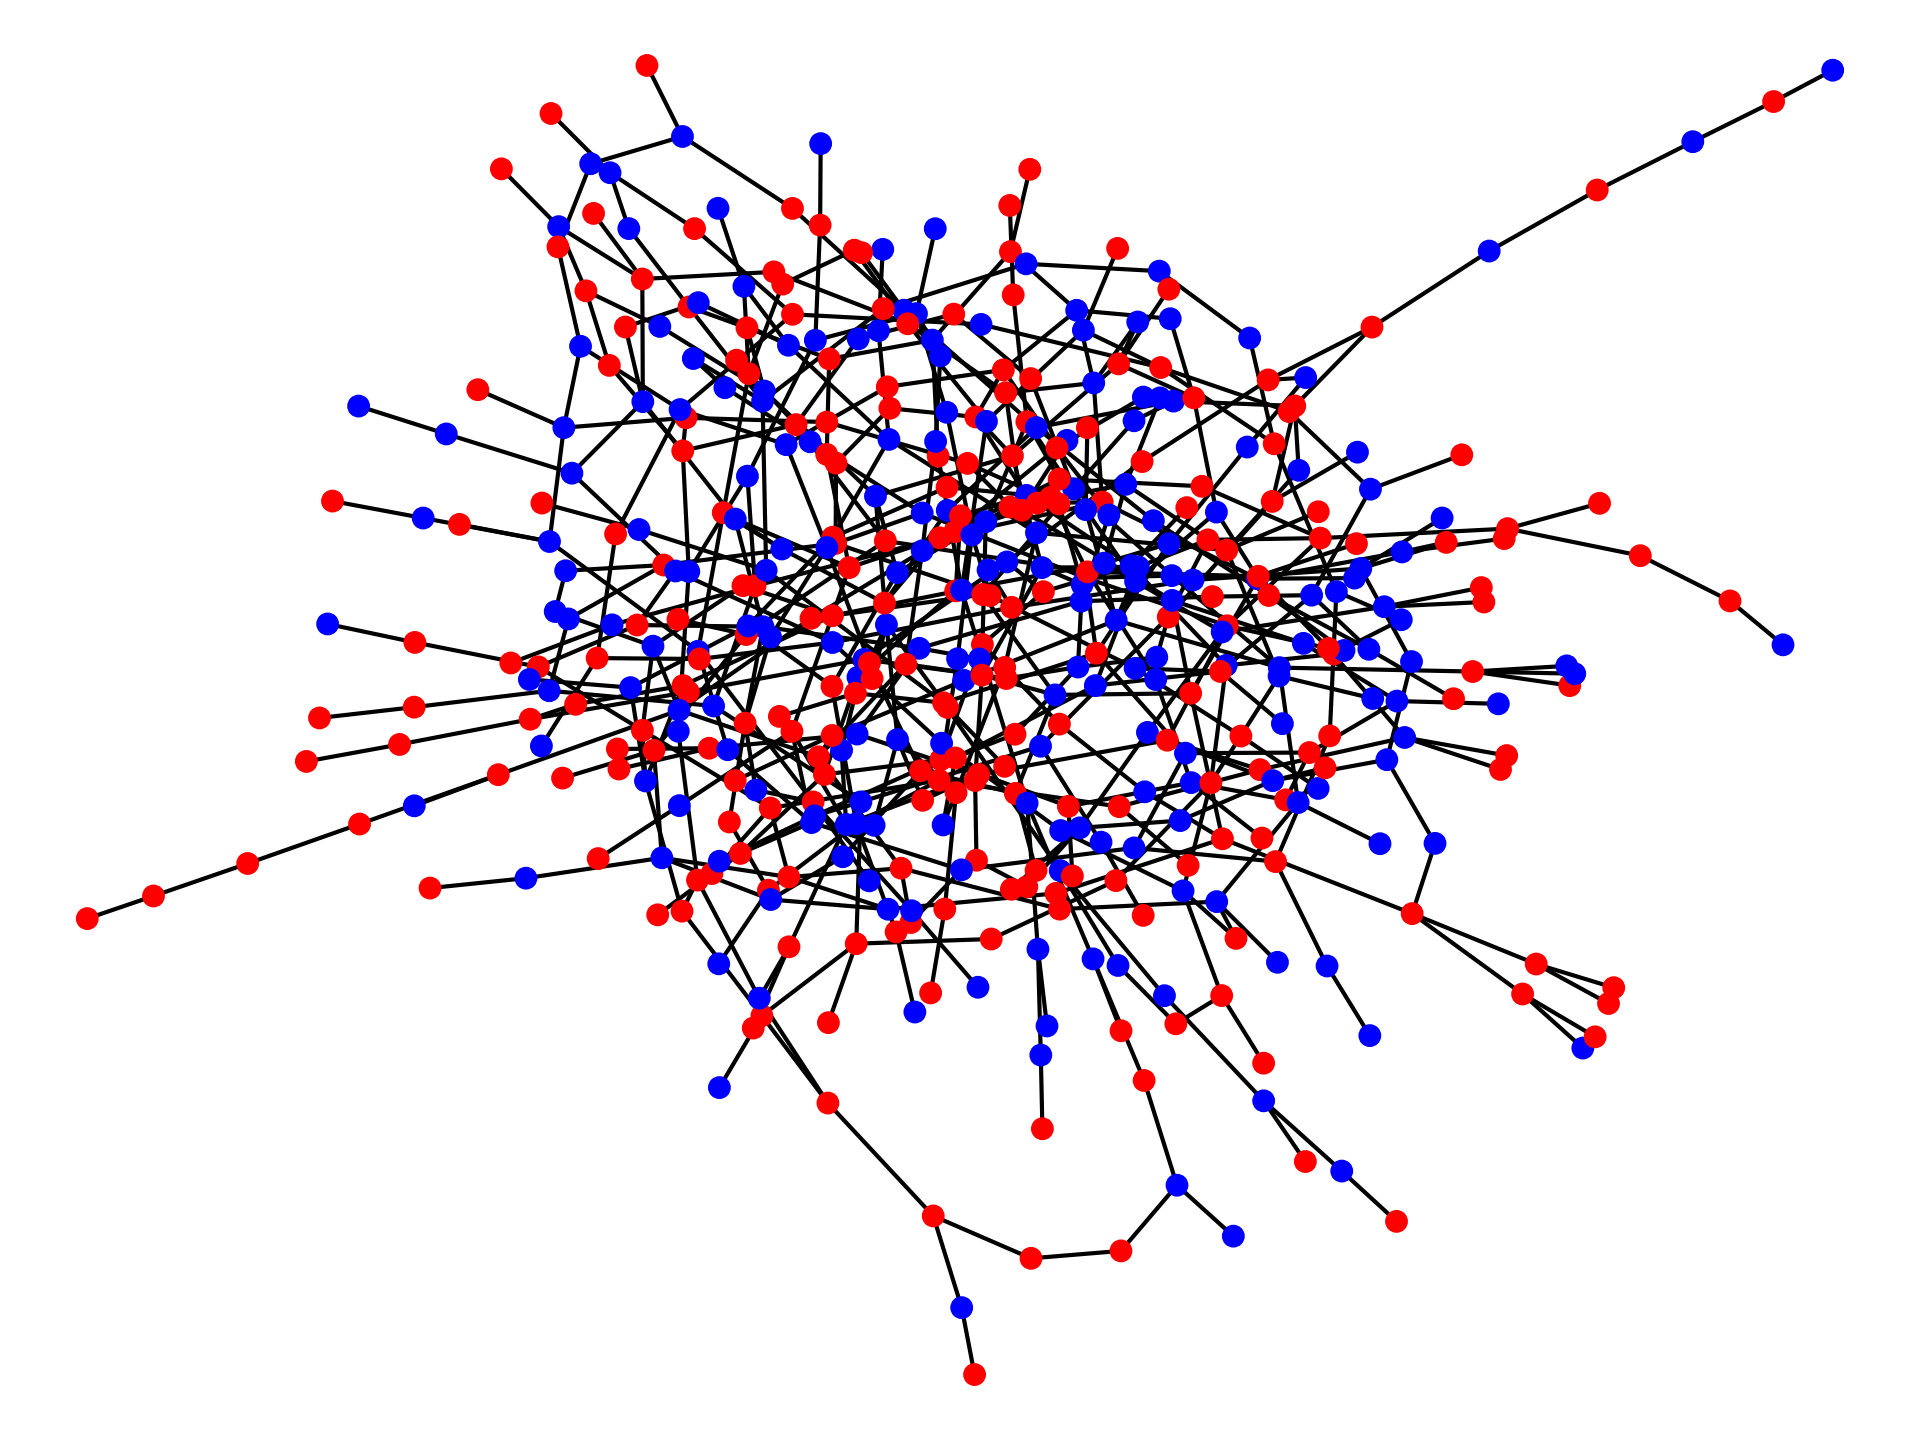
\includegraphics[scale=0.5]{images/example_network.png}
	\end{center}
	% $$\Pr(W=1) = 0.36,\; \Pr(A=1) = 0.47, \; \Pr(Y=1) = 0.68$$
\end{frame}

\begin{frame}{MossSpider}
	Available for Python 3.6+\footnote[frame]{Maintained at https://github.com/pzivich/MossSpider}\\
	\begin{center}
		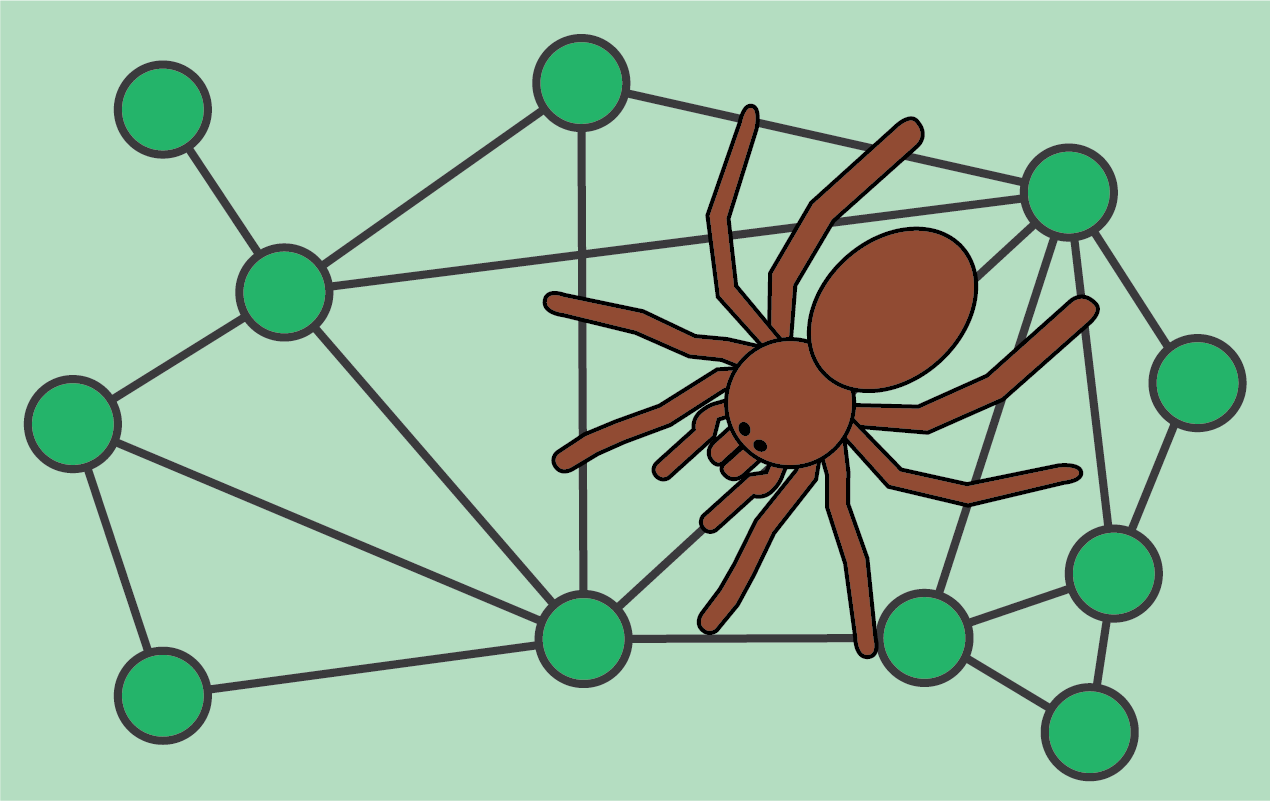
\includegraphics[scale=0.75]{images/mossspider_header.png}
	\end{center}
	\texttt{python -m pip install mossspider}
\end{frame}

\begin{frame}{Analysis with MossSpider}
	\inputpython{snah2022.py}{7}{7}

	\inputpython{snah2022.py}{48}{59}
\end{frame}

\begin{frame}{Analysis with MossSpider}
	\inputpython{snah2022.py}{66}{74}
\end{frame}

\begin{frame}{Results}
	\begin{center}
		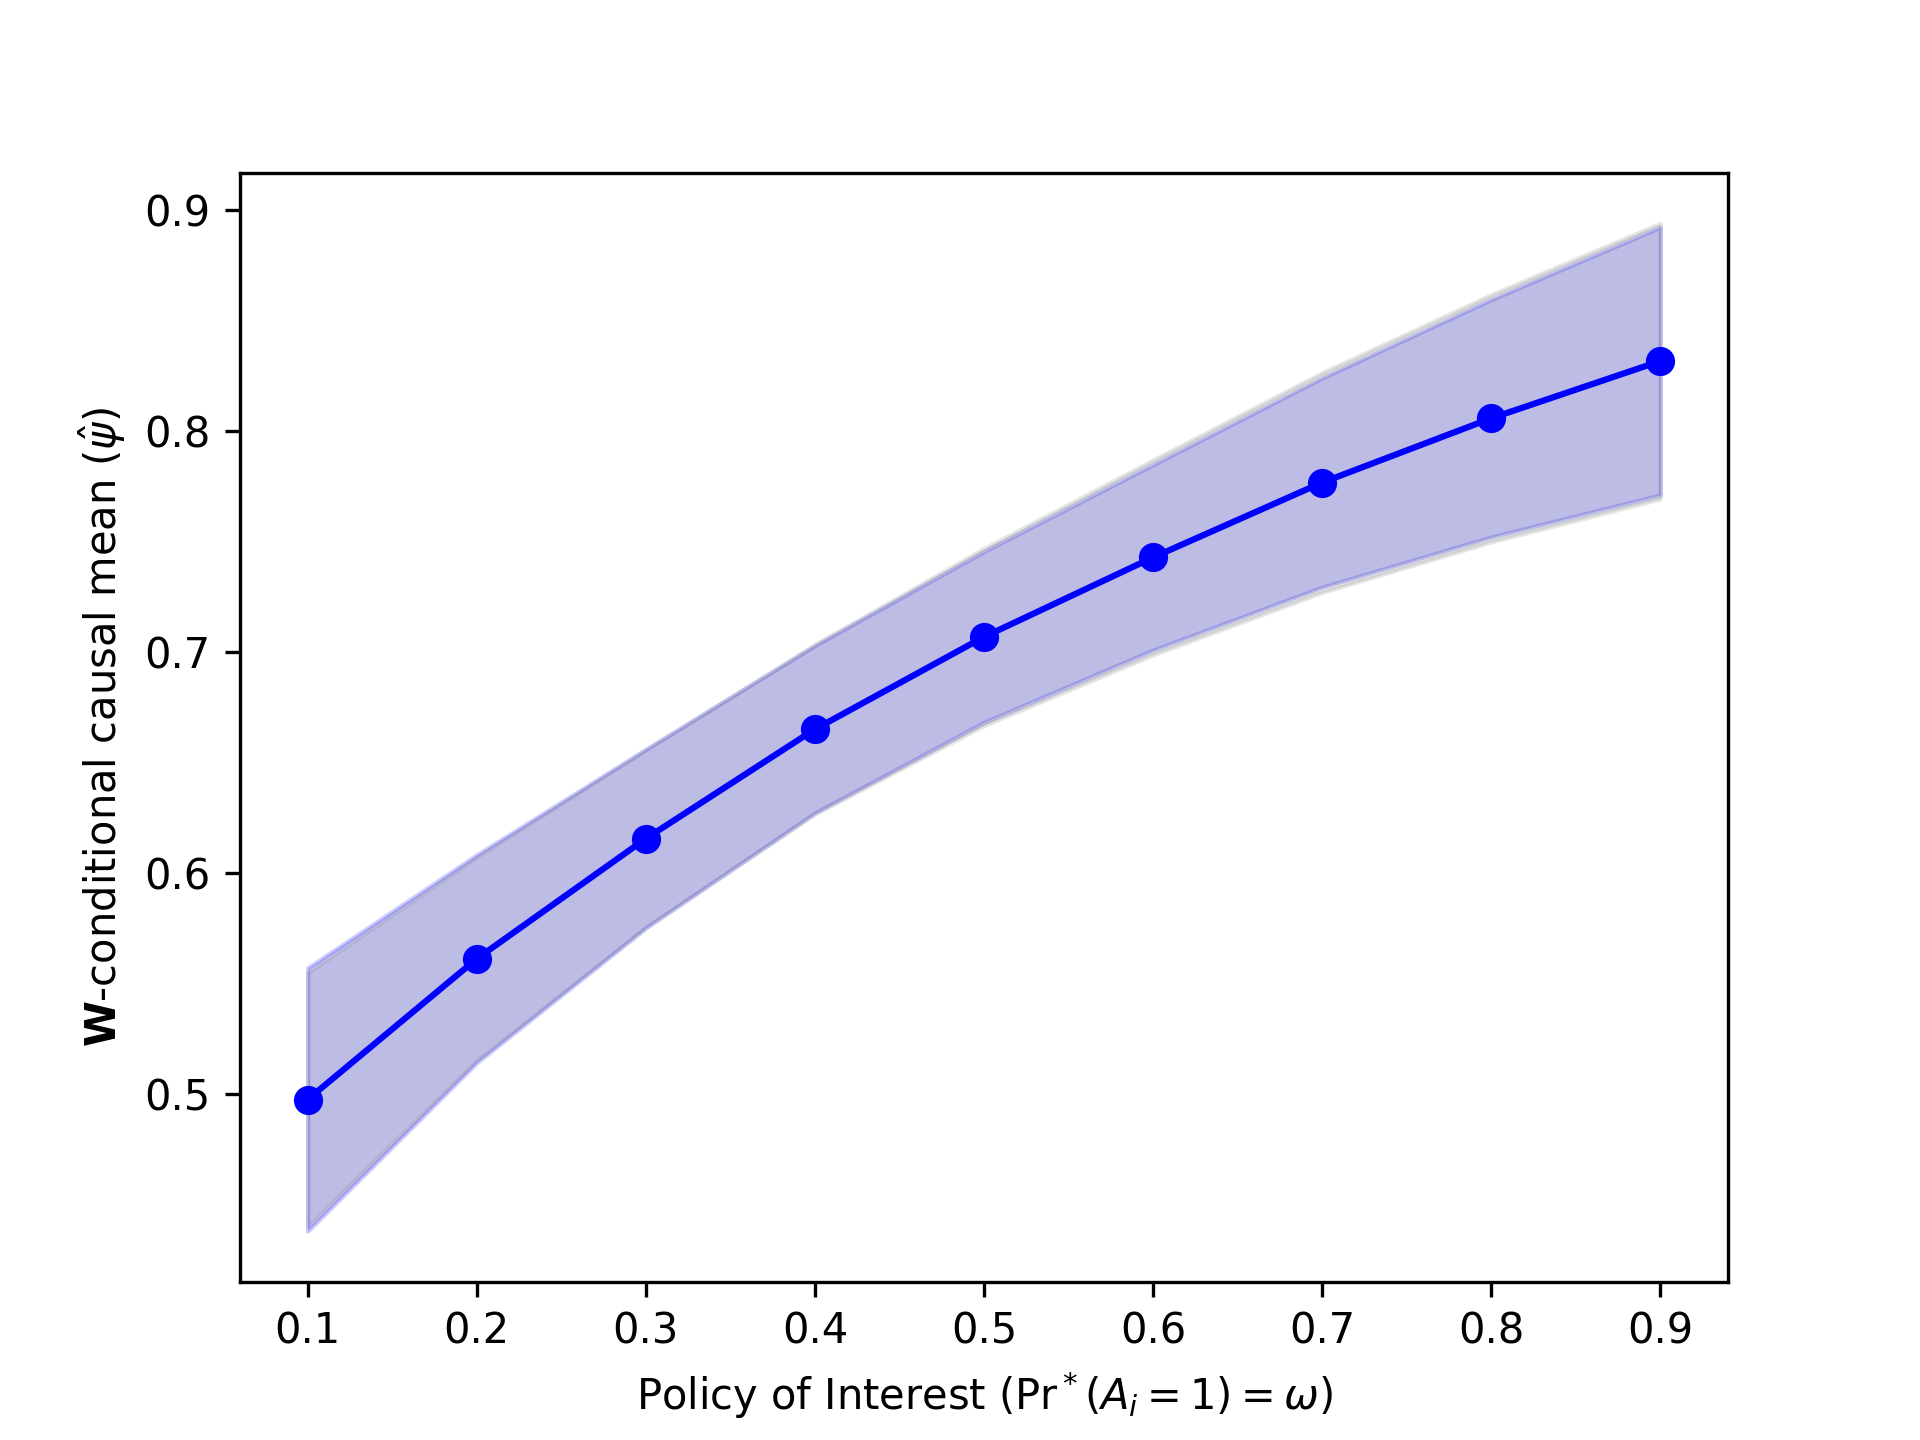
\includegraphics[scale=0.65]{images/example_results.png}
	\end{center}
\end{frame}

\section{Summary}

\begin{frame}{Summary}
	Causal inference with network data is difficult
	\begin{itemize}
		\item Unverifiable assumptions
		\item Simplifications of interference processes
	\end{itemize}~\\
	Network-TMLE
	\begin{itemize}
		\item One modern approach 
		\item Overview of how it works
		\item Implementation available in \texttt{mossspider}
	\end{itemize}
\end{frame}

\begin{frame}{References}
	\tiny
	Network-TMLE readings
	\begin{itemize}
		\item Ogburn EL, Sofrygin O, Diaz I, \& Van Der Laan MJ. (2017). "Causal inference for social network data". \textit{arXiv preprint} arXiv:1705.08527.
		\item Sofrygin O, \& van der Laan MJ. (2017). "Semi-parametric estimation and inference for the mean outcome of the single time-point intervention in a causally connected population". \textit{Journal of Causal Inference}, 5(1).
		\item van der Laan MJ. (2014). "Causal inference for a population of causally connected units". \textit{Journal of Causal Inference}, 2(1), 13-74.
	\end{itemize}
	Other resources
	\begin{itemize}
		\item Halloran ME, \& Hudgens MG. (2016). "Dependent happenings: a recent methodological review". \textit{Current Epidemiology Reports}, 3(4), 297-305.
		\item Hudgens MG, \& Halloran ME. (2008). "Toward causal inference with interference". \textit{Journal of the American Statistical Association}, 103(482), 832-842.
		\item Schuler MS, \& Rose S. (2017). "Targeted maximum likelihood estimation for causal inference in observational studies". \textit{American Journal of Epidemiology}, 185(1), 65-73.
		\item Snowden JM, Rose S, \& Mortimer KM. (2011). "Implementation of G-computation on a simulated data set: demonstration of a causal inference technique". \textit{American Journal of Epidemiology}, 173(7), 731-738.
		\item Westreich D, \& Cole SR. (2010). "Invited commentary: positivity in practice". \textit{American Journal of Epidemiology}, 171(6), 674-677.
		\item Zivich PN, \& Breskin A. (2021). "Machine learning for causal inference: on the use of cross-fit estimators". \textit{Epidemiology}, 32(3), 393-401.
		\item Zivich PN, Volfovsky A, Moody J, \& Aiello AE. (2021). "Assortativity and Bias in Epidemiologic Studies of Contagious Outcomes: A Simulated Example in the Context of Vaccination". \textit{American Journal of Epidemiology}, 190(11), 2442-2452.
	\end{itemize}
\end{frame}

\end{document}
